\documentclass{article}
\usepackage[english]{babel}
\usepackage[utf8]{inputenc}
\usepackage{amsmath,amssymb}
\usepackage{parskip}
\usepackage{graphicx}
\usepackage{dsfont}
\usepackage{dsfont}
\usepackage{relsize}
\usepackage{array}
\newcommand{\bigsigma}{\makebox{\Huge\ensuremath{\sigma}}}
\newcommand{\bigpi}{\makebox{\Huge\ensuremath{\Pi}}}
\newcolumntype{C}[1]{>{\centering\let\newline\\\arraybackslash\hspace{0pt}}m{#1}}
\usepackage[top=2.5cm, left=3cm, right=3cm, bottom=4.0cm]{geometry}
\usepackage[table]{xcolor}
\usepackage[utf8]{inputenc}
\usepackage{textcomp}
\usepackage[utf8]{inputenc}
\usepackage{amsmath}
\usepackage{amssymb}
\usepackage{xcolor}
\usepackage{listings}
\usepackage{xstring}
\usepackage{graphicx}
\usepackage[export]{adjustbox}

\definecolor{dkgreen}{rgb}{0,0.6,0}
\definecolor{ltgray}{rgb}{0.5,0.5,0.5}

\makeatletter
\newif\ifcolname
\colnamefalse

\def\keywordcheck{%
\IfStrEq*{\the\lst@token}{select}{\global\colnametrue}{}%
\IfStrEq*{\the\lst@token}{where}{\global\colnametrue}{}%
\IfStrEq*{\the\lst@token}{from}{\global\colnamefalse}{}%
\color{blue}%
}
\def\setidcolor{%
\ifcolname\color{purple}\else\color{black}\fi%
}
\makeatother

\lstset{%
    backgroundcolor=\color{white},
    basicstyle=\footnotesize,
    breakatwhitespace=false,
    breaklines=true,
    captionpos=b,
    commentstyle=\color{dkgreen},
    deletekeywords={...},
    escapeinside={\%*}{*)},
    extendedchars=true,
    frame=single,
    keepspaces=true,
    language=SQL,
    otherkeywords={is},
    morekeywords={*,modify,MODIFY,...},
    keywordstyle=\keywordcheck,
    identifierstyle=\setidcolor,
    numbers=left,
    numbersep=15pt,
    numberstyle=\tiny,
    rulecolor=\color{ltgray},
    showspaces=false,
    showstringspaces=false, 
    showtabs=false,
    stepnumber=1,
    tabsize=4,
    title=\lstname
}

\newcommand{\tablespace}{\\[1.25mm]}
\newcommand\Tstrut{\rule{0pt}{2.6ex}}         % = `top' strut
\newcommand\tstrut{\rule{0pt}{2.0ex}}         % = `top' strut
\newcommand\Bstrut{\rule[-0.9ex]{0pt}{0pt}}   % = `bottom' strut
\title{Assignment-5 CS313}
\author{Shashank P \\ 200010048}
\date{\today}

\begin{document}
\maketitle




\section{Part A}
\subsection{Problem 1}
Using the handout (JDBC Handout.pdf) which is uploaded on moodle, try out the
java+jdbc code.
\begin{figure}[!ht]
  \begin{center}
  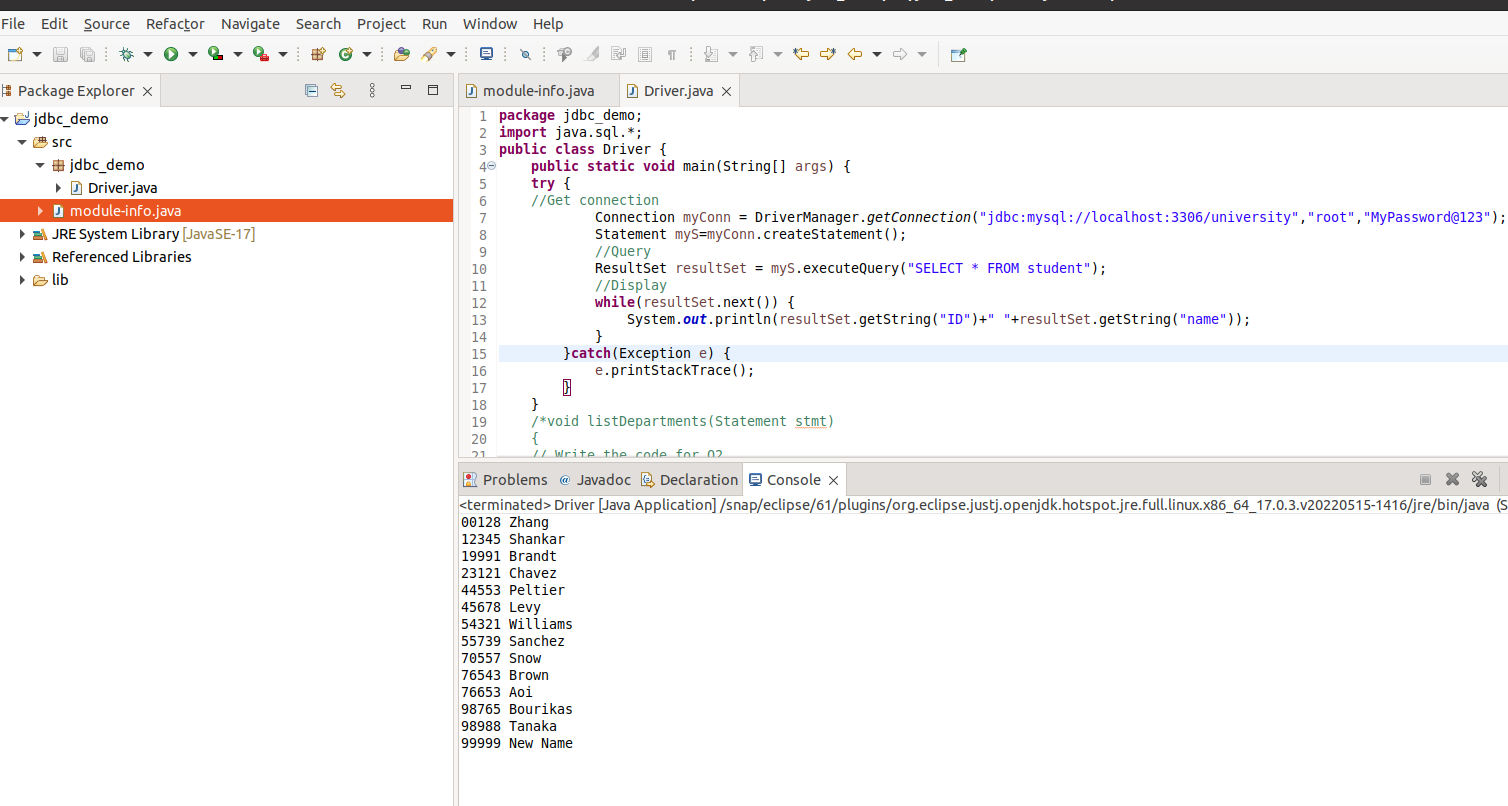
\includegraphics[scale=0.5]{Part_A_1.png}
  \caption{Program Output}
  \end{center}
\end{figure}

\newpage
\subsection{Problem 2}
Modify the code given to you to list departments (in asc order) and the total number of
students and instructors they have. A template has been made in the provided source
code(Driver.java), you need to fill up the template.
\begin{lstlisting}[language=sql]
WITH S_count(dname, s_count) AS
  (SELECT S.dept_name, count(*)
  FROM student S
  GROUP BY S.dept_name),
I_count(dname, i_count) AS
  (SELECT I.dept_name, count(*)
  FROM instructor I
  GROUP BY I.dept_name)
SELECT *
FROM I_count LEFT OUTER JOIN S_count
ON I_count.dname=S_count.dname
UNION
SELECT *
FROM I_count RIGHT OUTER JOIN S_count
ON I_count.dname=S_count.dname
\end{lstlisting}
\begin{figure}[!ht]
  \begin{center}
  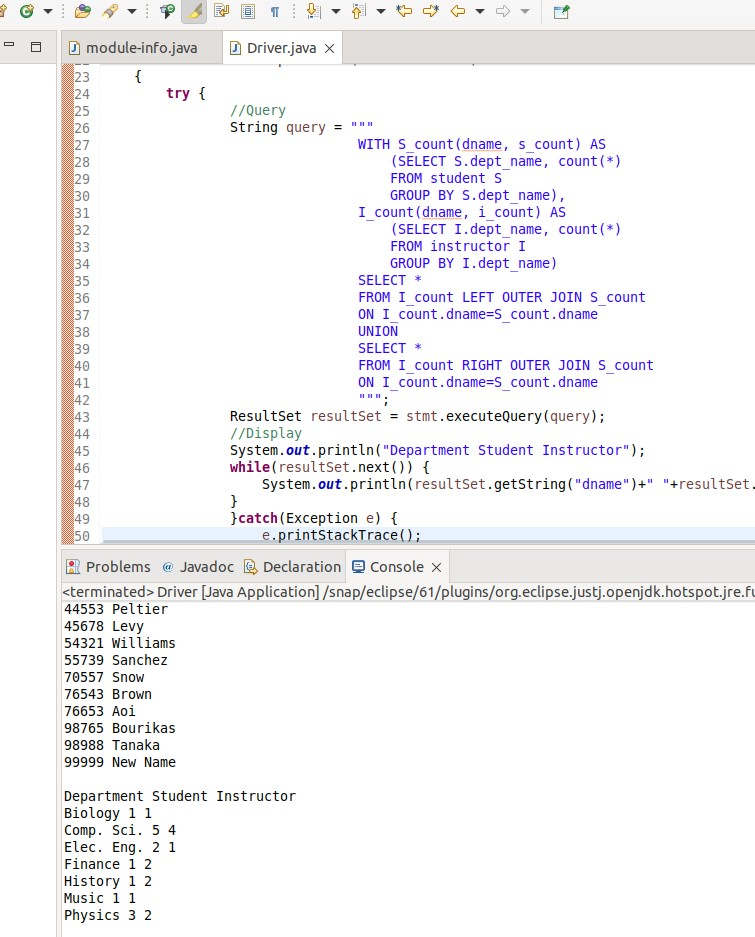
\includegraphics[scale=0.5]{Part_A_2.jpg}
  \caption{Program Output}
  \end{center}
\end{figure}

\newpage
\subsection{Problem 3}
Do the following preparedStatement : For a given building, find classrooms (room\_no)
with capacity more than 30 and in which no courses are scheduled this year and semester.
A template has been made in the provided source code(Driver.java), you need to fill up
the template.
\begin{lstlisting}[language=sql]
select distinct class.room_number 
from classroom class natural join section sec 
where capacity>30 and class.room_number NOT IN 
(select room.room_number from classroom room 
natural join section sect 
where capacity>30 and sect.semester='Fall' and sect.year=2009);
\end{lstlisting}
\begin{figure}[!ht]
  \begin{center}
  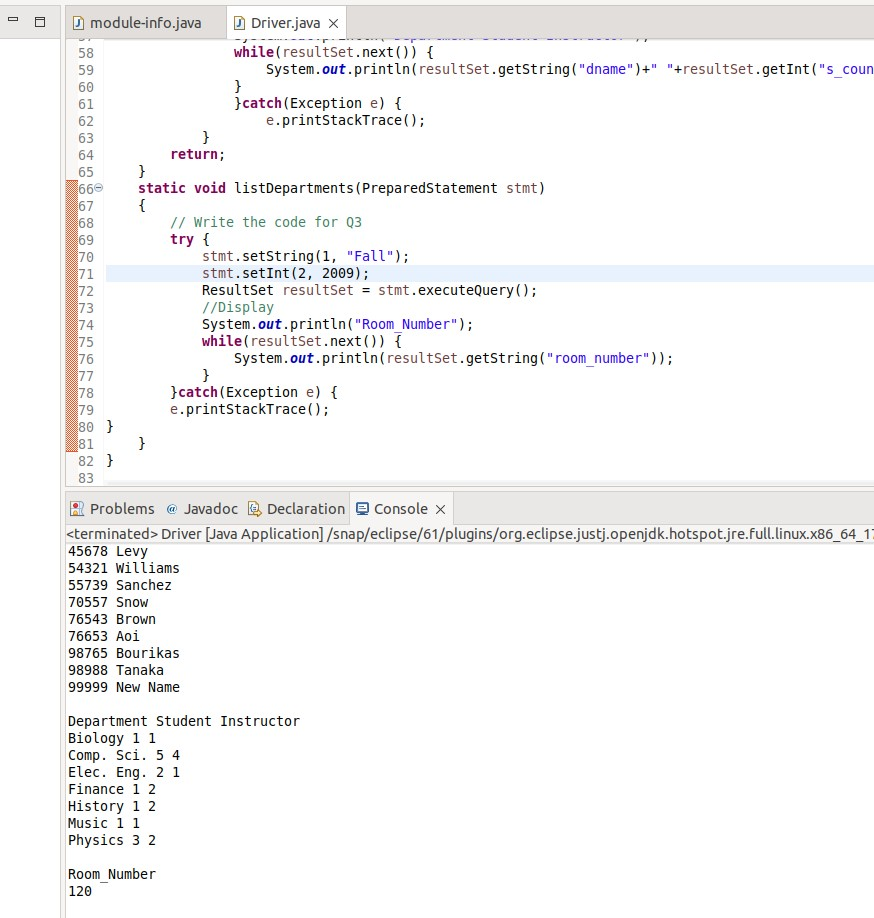
\includegraphics[scale=0.5]{Part_A_3.jpg}
  \caption{Program Output}
  \end{center}
\end{figure}


\newpage
\section{Part 2}
Design a new html page to take advisor id as input. Write a servlet to display the
department to which the advisor belongs using the Java and J2EE program. Output
should contain advisor id and department name.
\begin{figure}[!ht]
  \begin{center}
  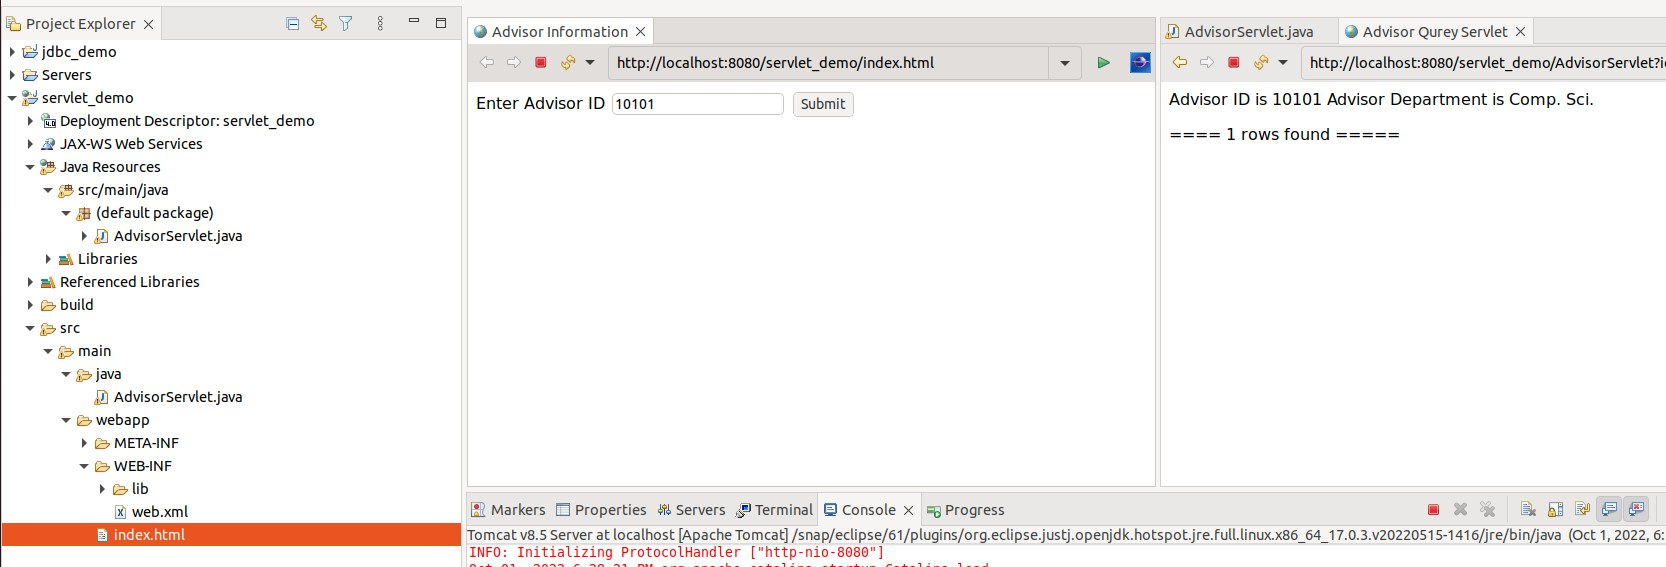
\includegraphics[scale=0.4]{Part_B_1.jpg}
  \caption{Servlet Output}
  \end{center}
\end{figure}

\end{document}
